Der Projektstrukturplan zeigt hierarchisch gegliedert alle plan- und kontrollierbaren Teilaufgaben. Diese Teilaufgaben entstehen dadurch, indem die Gesamtaufgabe des Projektes so lange in kleinere Arbeitspakete aufgeteilt wird, bis eine weitere Aufteilung nicht mehr sinnvoll wäre. Durch die hierarchische Struktur entstehen Ebenen, in die das Projekt aufgeteilt ist. Die oberste Ebene ist die Allgemeinheit des Projekts, betitelt mit dem Projektnamen. Darunter befinden sich die Phasen und unter diesen befinden sich besagte Arbeitspakete. Jeder dieser Punkte hat seinen eigenen, eindeutigen PSP-Code.
\\Der \enquote{PSP} stellt auch die Grundlage für weitere relevante Planungsschritte im Projektmanagement dar, wie beispielsweise Terminpläne, Ressourcenpläne und Kostenpläne \cite{Kindl_Niels:2023}.

\begin{figure}[H]
	\centering
	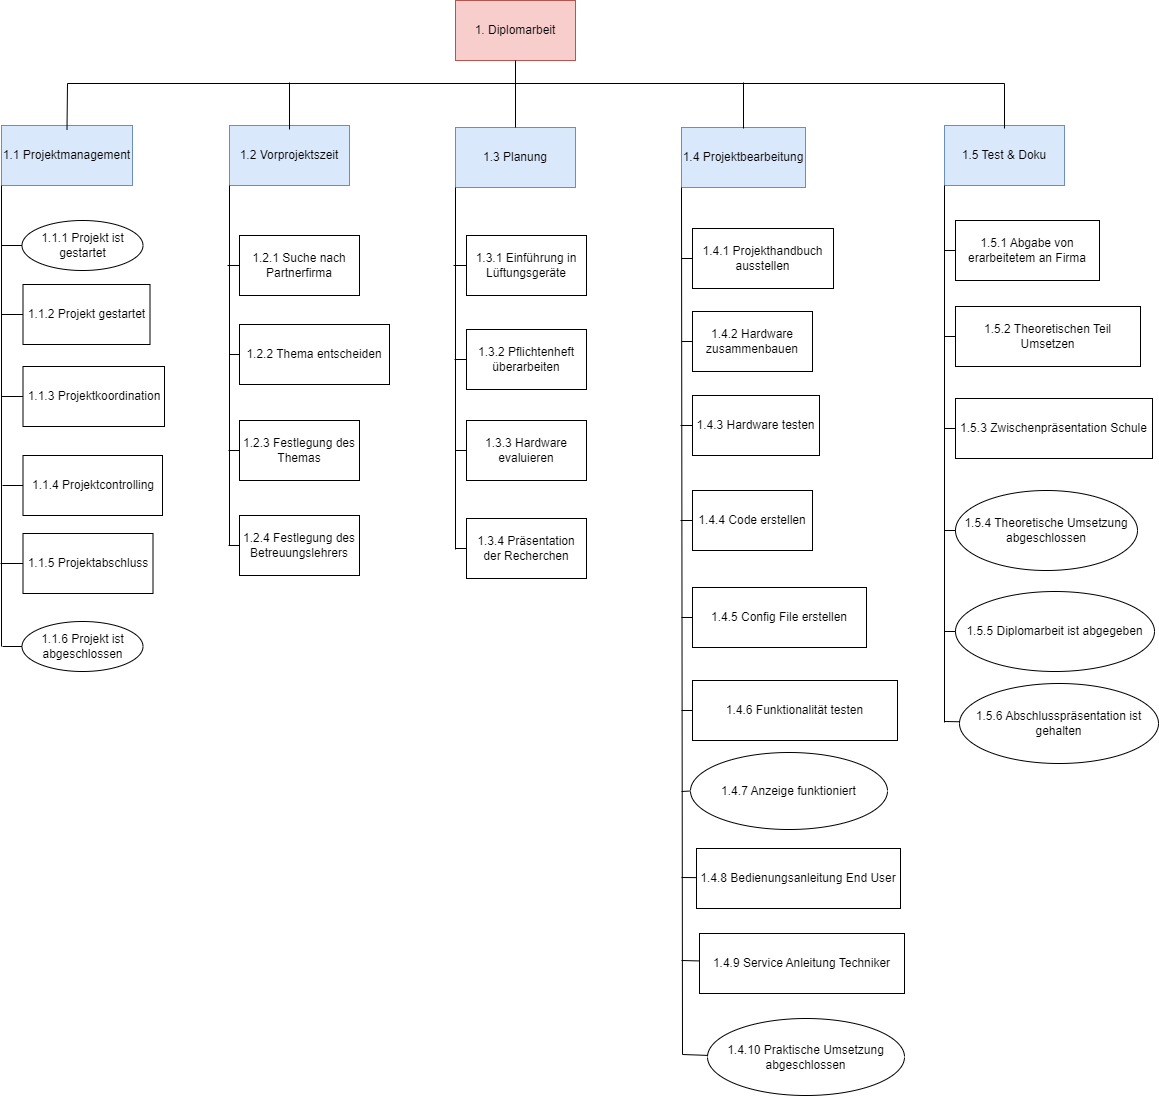
\includegraphics[width=1\linewidth]{Bilder/projektstrukturplan}
	\caption{Projektstukturplan}
	\label{fig:projektstrukturplan}
\end{figure}